\subsection{Example~3.5}



\subsubsection{General Observations}

Sawtooth functions correspond to sequences of numbers
\[
	0 < s_1 < r_1 < s_2 < r_2 < \dotsb < s_n < r_n < 1 \,,
\]
where~$n ≥ 1$, the numbers~$r_1, \dotsc, r_n$ are the positions of the vertices, and the numbers~$s_1, \dotsc, s_n$ are the positions of the spikes, see \cref{parametrization of sawtooth functions}.
\begin{figure}
	\centering
	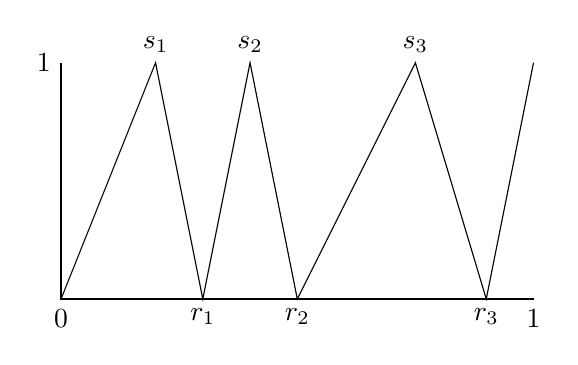
\begin{tikzpicture}[scale = 3, xscale = 2]
		% axis
			\draw[thick] (0, 1) node[left]{$1$} -- (0, 0) node[below]{$0$} -- (1, 0) node[below]{$1$};
		% the line
		\draw (0, 0)
		-- (0.2 , 1) node[above] {$s_1$}
		-- (0.3 , 0) node[below] {$r_1$}
		-- (0.4 , 1) node[above] {$s_2$}
		-- (0.5 , 0) node[below] {$r_2$}
		-- (0.75, 1) node[above] {$s_3$}
		-- (0.9 , 0) node[below] {$r_3$}
		-- (1.0 , 1);
	\end{tikzpicture}
	\caption{Parametrization of sawtooth functions by its vertices and spikes.}
	\label{parametrization of sawtooth functions}
\end{figure}

To describe the closure of~$A$, we will use the following interpolation result.

\begin{proposition}[Interpolation by Sawtooth Functions]
	\label{interpolation via sawtooth functions}
	Let~$n ≥ 1$ be a number of data points, let~$0 < x_1 < \dotsb < x_n < 1$ and let~$y_1, \dotsc, y_n ∈ [0, 1]$.
	There exists a sawtooth function~$f \colon [0, 1] \to [0, 1]$ with~$f x_i = y_i$ for every~$i = 1, \dotsc, n$.
\end{proposition}

\begin{proof}
	Suppose we are given some~$0 < x < 1$ and some~$0 < y < 1$.
	Given~$δ > 0$, there exists a unique line going through the points~$(x - δ, 1)$ and~$(x, y)$.
	This unique line intersects the horizontal line~$ℝ × \{ 1 \}$ at precisely one point, which is of the form~$(x + δ', 0)$ for some~$δ' > 0$, as depicted in \cref{graphical justification for slope formula}.
	We have
	\[
		\frac{y}{δ'} = \frac{1 - y}{δ} \,,
	\]
	and therefore
	\[
		δ' = \frac{y}{1 - y} \, δ \,.
	\]
	\begin{figure}
		\centering
		\begin{tikzpicture}[scale = 3.5, xscale = 1.5];
			% axes
			\draw[thick] (-0.1, 0) node[left] {$0$} -- (1.1, 0);
			\draw[thick] (-0.1, 1) node[left] {$1$} -- (1.1, 1);
			% points
			\draw[fill] (0.2, 1)   ellipse (0.015 and 0.0225) node[above] {$\rightarrow$};
			\draw[fill] (0.5, 0.4) ellipse (0.015 and 0.0225);
			\draw[fill] (0.7, 0)   ellipse (0.015 and 0.0225) node[below] {$\leftarrow$};
			% lines
			\draw (0.5, 0) --node[left] {$y$} (0.5, 0.4) --node[right] {$1 - y$}  (0.5, 1) node[above] {$x$};
			\draw (0.7, 0) -- (0.2, 1);
			% non-visible lines for placement of deltas
			\draw (0.2, 1) --node[above] {$δ$}  (0.5, 1);
			\draw (0.5, 0) --node[below] {$δ'$} (0.7, 0);
		\end{tikzpicture}
		\caption{We have~$y / δ = (1 - y) / δ'$, and as~$δ \to 0$ we also have~$δ' \to 0$.}
		\label{graphical justification for slope formula}
	\end{figure}
	So for~$δ \to 0$ we have also~$δ' \to 0$.

	Let now~$ε > 0$ such that the intervals~$(x_i - ε, x_i + ε)$ are contained in~$[0, 1]$ and pairwise disjoint.
	We define the values~$s_i$ and~$r_i$ as follows:
	\begin{casedistinction}

		\item
			If~$y_i = 0$ then~$s_i ≔ (x_i - ε/2, 1)$ and~$r_i ≔ (x_i, 0) = (x_i, y_i)$.

		\item
			If~$y_i = 1$ then~$s_i ≔ (x_i, 1) = (x_i, y_i)$ and~$r_i ≔ (x_i  + ε/2, 0)$.

		\item
			If~$0 < y_i < 1$, then let~$δ > 0$ be sufficiently small so that both~$δ < ε$ and also~$δ' < ε$ for~$δ' ≔ y / (y - 1) ⋅ δ$.
			We then set~$s_i ≔ (x_i - δ, 1)$ and~$r_i ≔ (x_i + δ', 0)$.

	\end{casedistinction}
	The sawtooth function~$f$ corresponding to the numbers
	\[
		0 < s_1 < r_1 < \dotsb < s_n < r_n < 1
	\]
	satisfies~$f x_i = y_i$ for every~$i = 1, \dotsc, n$.
	See \cref{interpolationg sawtooth function} for an example.
	\begin{figure}
		\[
			\begin{array}{crcr}
				{}
				&
				\centerbox{
				\begin{tikzpicture}[scale = 2.5, xscale = 2]
					% gray areas
					%\draw[fill, gray!30] (0.1, 1) rectangle (0.3, 0);
					%\draw[fill, gray!30] (0.4, 1) rectangle (0.6, 0);
					%\draw[fill, gray!30] (0.7, 1) rectangle (0.9, 0);
					% axes
					\draw[thick] (0, 1) -- (0, 0) -- (1, 0);
					% the points to be interpolated
					\draw[fill] (0.2, 0)   ellipse (0.015 and 0.03);
					\draw[fill] (0.5, 0.5) ellipse (0.015 and 0.03);
					\draw[fill] (0.8, 1)   ellipse (0.015 and 0.03);
					% the intervals with ε = 0.1
					%\draw[(-)] (0.1, -0.2) -- (0.3, -0.2);
					%\draw[(-)] (0.4, -0.2) -- (0.6, -0.2);
					%\draw[(-)] (0.7, -0.2) -- (0.9, -0.2);
				\end{tikzpicture}
				}
				&
				\leadsto
				&
				\centerbox{
				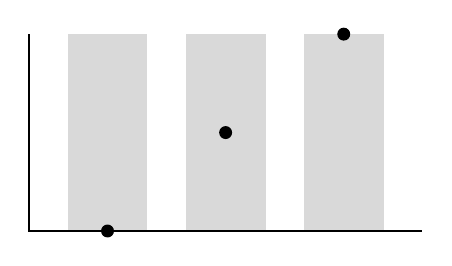
\begin{tikzpicture}[scale = 2.5, xscale = 2]
					% gray areas
					\draw[fill, gray!30] (0.1, 1) rectangle (0.3, 0);
					\draw[fill, gray!30] (0.4, 1) rectangle (0.6, 0);
					\draw[fill, gray!30] (0.7, 1) rectangle (0.9, 0);
					% axes
					\draw[thick] (0, 1) -- (0, 0) -- (1, 0);
					% the points to be interpolated
					\draw[fill] (0.2, 0)   ellipse (0.015 and 0.03);
					\draw[fill] (0.5, 0.5) ellipse (0.015 and 0.03);
					\draw[fill] (0.8, 1)   ellipse (0.015 and 0.03);
					% the intervals with ε = 0.1
					%\draw[(-)] (0.1, -0.2) -- (0.3, -0.2);
					%\draw[(-)] (0.4, -0.2) -- (0.6, -0.2);
					%\draw[(-)] (0.7, -0.2) -- (0.9, -0.2);
				\end{tikzpicture}
				}
				\\[5em]
				\leadsto
				&
				\centerbox{
				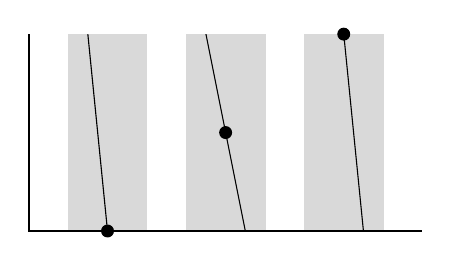
\begin{tikzpicture}[scale = 2.5, xscale = 2]
					% gray areas
					\draw[fill, gray!30] (0.1, 1) rectangle (0.3, 0);
					\draw[fill, gray!30] (0.4, 1) rectangle (0.6, 0);
					\draw[fill, gray!30] (0.7, 1) rectangle (0.9, 0);
					% axes
					\draw[thick] (0, 1) -- (0, 0) -- (1, 0);
					% the points to be interpolated
					\draw[fill] (0.2, 0)   ellipse (0.015 and 0.03);
					\draw[fill] (0.5, 0.5) ellipse (0.015 and 0.03);
					\draw[fill] (0.8, 1)   ellipse (0.015 and 0.03);
					% the intervals with ε = 0.1
					%\draw[(-)] (0.1, -0.2) -- (0.3, -0.2);
					%\draw[(-)] (0.4, -0.2) -- (0.6, -0.2);
					%\draw[(-)] (0.7, -0.2) -- (0.9, -0.2);
					% lines
					\draw (0.15, 1) -- (0.2,  0);
					\draw (0.45, 1) -- (0.55, 0);
					\draw (0.8,  1) -- (0.85, 0);
				\end{tikzpicture}
				}
				&
				\leadsto
				&
				\centerbox{
				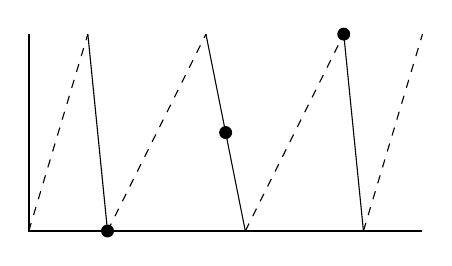
\begin{tikzpicture}[scale = 2.5, xscale = 2]
					% gray areas
					%\draw[fill, gray!30] (0.1, 1) rectangle (0.3, 0);
					%\draw[fill, gray!30] (0.4, 1) rectangle (0.6, 0);
					%\draw[fill, gray!30] (0.7, 1) rectangle (0.9, 0);
					% axes
					\draw[thick] (0, 1) -- (0, 0) -- (1, 0);
					% the points to be interpolated
					\draw[fill] (0.2, 0)   ellipse (0.015 and 0.03);
					\draw[fill] (0.5, 0.5) ellipse (0.015 and 0.03);
					\draw[fill] (0.8, 1)   ellipse (0.015 and 0.03);
					% the intervals with ε = 0.1
					%\draw[(-)] (0.1, -0.2) -- (0.3, -0.2);
					%\draw[(-)] (0.4, -0.2) -- (0.6, -0.2);
					%\draw[(-)] (0.7, -0.2) -- (0.9, -0.2);
					% lines
					\draw (0.15, 1) -- (0.2,  0);
					\draw (0.45, 1) -- (0.55, 0);
					\draw (0.8,  1) -- (0.85, 0);
					\draw[dashed] (0,    0) -- (0.15, 1);
					\draw[dashed] (0.2,  0) -- (0.45, 1);
					\draw[dashed] (0.55, 0) -- (0.8,  1);
					\draw[dashed] (0.85, 0) -- (1,    1);
				\end{tikzpicture}
				}
			\end{array}
		\]
		\caption{A sawtooth function that interpolated between for the three points~$(0.2, 0)$,~$(0.5, 0.5)$ and~$(0.8, 1)$.}
		\label{interpolationg sawtooth function}
	\end{figure}
\end{proof}



\subsubsection{The Closure of~$A$}

Instead of only showing that the zero function lies in the closure in~$A$, we show more generally that~$A$ is dense in~$X$.
To this end, we characterize dense subsets in terms of their intersection with open sets:

\begin{lemma}
	Let~$X$ be a topological space and let~$D$ be a subset of~$X$.
	The set~$D$ is dense in~$X$ if and only if every nonempty open subset of~$X$ intersects~$D$.
\end{lemma}

In other words:
the definition of \enquote{dense} we gave in \cref{definition of dense subsets} is equivalent to the definition given in Section~3.1 the book.

\begin{proof}
	We have the chain of equivalences
	\begin{align*}
		{}&
		\text{$D$ is dense in~$X$} \\
		\iff{}&
		\closure{D} = X \\
		\iff{}&
		\text{the only closed subset of~$X$ that contains~$D$ is~$X$ itself} \\
		\iff{}&
		\text{the only open subset of~$X$ that doesn’t intersect~$D$ is~$∅$} \,,
	\end{align*}
	which proves the assertion.
\end{proof}

Let now~$U$ be any nonempty open subset of~$[0, 1]^{[0, 1]}$.
We need to show that~$A$ intersects~$U$.
For this, we may assume that~$U$ is a basic open set for the product topology, i.e., that there exist distinct points~$x_1, \dotsc, x_n$ in~$[0, 1]$ and open subsets~$U_1, \dotsc, U_n$ of~$[0, 1]$ with
\[
	U
	=
	\{
		f ∈ [0, 1]^{[0, 1]}
		\suchthat
		\text{$f x_i ∈ U_i$ for every~$i$}
	\} \,.
\]
The neighbourhood~$U$ is nonempty, so the sets~$U_i$ must also be nonempty.
For every index~$i$ we choose some point~$y_i$ in~$U_i$.
We know from \cref{interpolation via sawtooth functions} that there exist a sawtooth function~$f$ with~$f x_i = y_i$ for every~$i$, and thus~$f ∈ U$.
This shows that~$U$ intersects~$A$.



\subsubsection{The Zero Function is Not The Limit of a Sequence in~$A$}

\begin{proposition}
	\label{convergece of sequences in products is coordinate-wise}
	Let~$(X_α)_{α ∈ A}$ be a family of topological spaces, let~$(x_n)_n$ be a sequence in~$X ≔ ∏_{α ∈ A} X_α$, and let~$x$ be some point in~$X$.
	Then~$(x_n)_n \to x$ in~$X$ if and only if this holds in each coordinate.
	More explicitly, if~$x_n = (x_n^α)_α$ and~$x = (x^α)_α$, then~$(x_n)_n \to x$ if and only if~$(x_n^α)_α \to x^α$ for every index~$α ∈ A$.
\end{proposition}

\begin{proof}
	For all distinct indices~$α_1, \dotsc, α_r ∈ A$ and all open subsets~$U_i ⊆ X_{α_i}$ we denote the resulting basic open subset of~$X$ by
	\[
		P(U_1, \dotsc, U_r)
		≔
		∏_{α ∈ A}
		\begin{cases*}
			U_i & if~$α = α_i$ for some~$i$, \\
			X_α & otherwise.
		\end{cases*}
	\]
	We have the chain of equivalences
	\begingroup
	\allowdisplaybreaks
	\begin{align*}
		{}&
		(x_n)_n \to x
		\\
		\iff{}&
		\left\{
		\begin{tabular}{l}
			for every open subset~$U$ of~$X$ with~$x ∈ U$, \\
			there exists some~$N$ with~$x_n ∈ U$ for every~$n ≥ N$
		\end{tabular}
		\right.
		\\
		\iff{}&
		\left\{
		\begin{tabular}{l}
			for every basic open subset~$U$ of~$X$ with~$x ∈ U$, \\
			there exists some~$N$ with~$x_n ∈ U$ for every~$n ≥ N$
		\end{tabular}
		\right.
		\\
		\iff{}&
		\left\{
		\begin{tabular}{l}
			for all distinct indices~$α_1, \dotsc, α_r ∈ A$ \\
			and open subsets~$U_i ⊆ X_{α_i}$ with~$x ∈ P(U_1, \dotsc, U_r)$, \\
			there exists some~$N$ with~$x_n ∈ P(U_1, \dotsc, U_r)$ for every~$n ≥ N$
		\end{tabular}
		\right.
		\\
		\iff{}&
		\left\{
		\begin{tabular}{l}
			for all distinct indices~$α_1, \dotsc, α_r ∈ A$ \\
			and open subsets~$U_i ⊆ X_{α_i}$ with~$x^{α_i} ∈ U_i$ for every~$i$, \\
			there exists some~$N$ with~$x_n^{α_i} ∈ U_i$ for all~$i$ and~$n ≥ N$
		\end{tabular}
		\right.
		\\
		\iff{}&
		\left\{
		\begin{tabular}{l}
			for all distinct indices~$α_1, \dotsc, α_r ∈ A$ \\
			and open subsets~$U_i ⊆ X_{α_i}$ with~$x^{α_i} ∈ U_i$ for every~$i$, \\
			there exists some~$N_1, \dotsc, N_r$ with~$x_n^{α_i} ∈ U_i$ for all~$i$ and ~$n ≥ N_i$
		\end{tabular}
		\right.
		\\
		\iff{}&
		\left\{
		\begin{tabular}{l}
			for every index~$α ∈ A$ \\
			and every open subset~$U ⊆ X_α$ with~$x^α ∈ U$, \\
			there exists some~$N$ with~$x_n^α ∈ U$ for every~$n ≥ N$
		\end{tabular}
		\right.
		\\
		\iff{}&
		\text{$(x_n^α)_n \to x^α$ for every~$α ∈ A$} \,.
	\end{align*}
	\endgroup
	This shows the claimed equivalence.
\end{proof}

Suppose there exists a sequence of sawtooth functions~$(f_n)_n$ with~$(f_n)_n \to 0$ with respect to the product topology on~$[0, 1]^{[0, 1]}$.
According to the above \lcnamecref{convergece of sequences in products is coordinate-wise} this is equivalent to~$(f_n)_n \to 0$ pointwise.
However, we will see in the following that this cannot happen, since sawtooth functions are rather rigid:
not too many values of~$f_n$ can tend to~$0$ at the same time.

There exists by assumption for every point~$x$ in~$[0, 1]$ some natural number~$N$ such that~$f_n x ≤ 1/2$ for every~$n ≥ N$.
For every natural number~$N$ let
\[
	B_N
	≔
	\{ x ∈ [0, 1] \suchthat \text{$f_n x ≤ 1/2$ for every~$n ≥ N$} \} \,.
\]
These sets~$B_N$ form an increasing filtration of~$[0, 1]$, i.e., we have
\[
	B_0 ⊆ B_1 ⊆ B_2 ⊆ B_3 ⊆ \dotsb
\]
and~$[0, 1] = ⋃_{N = 0}^∞ B_N$.
We can also describe the sets~$B_N$ in terms of the sets
\[
	B'_n ≔ \{ x ∈ [0, 1] \suchthat f_n x ≤ 1/2 \}
\]
as the intersection~$B_N = ⋂_{n ≥ N} B'_n$.

We note that each set~$B'_n$ is Lebesgue-measurable, since the sawtooth function~$f_n$ is continuous.
Let us calculate the Lebesgue-measure of~$B'_n$:

We observe that for every sawtooth function~$f$ with corresponding points
\[
	0 < s_1 < r_1 < s_2 < r_2 < \dotsb < s_n < r_n < 1 \,,
\]
we have for the set~$B' ≔ \{ x ∈ [0, 1] \suchthat f x ≤ 1/2 \}$ the explicit description
\[
	B'
	=
	\biggl[ 0, \frac{s_1}{2} \biggr]
	∪ \biggl[ \frac{s_1 + r_1}{2}, \frac{r_1 + s_2}{2} \biggr]
	∪ \biggl[ \frac{s_2 + r_2}{2}, \frac{r_2 + s_3}{2} \biggr]
	∪ \dotsb
	∪ \biggl[ \frac{s_n + r_n}{2}, \frac{r_n + 1}{2} \biggr] \,.
\]
See \cref{cutting sawtooth function in half} for a visualization.
\begin{figure}
	\centering
	\begin{tikzpicture}[scale = 3, xscale = 4]
		% coordinates
		\coordinate (0)  at (0,    0);
		\coordinate (s1) at (0.2,  0);
		\coordinate (r1) at (0.3,  0);
		\coordinate (s2) at (0.4,  0);
		\coordinate (r2) at (0.5,  0);
		\coordinate (s3) at (0.75, 0);
		\coordinate (r3) at (0.9,  0);
		% coloured areas
		\draw[fill, gray!50] (0, 0) -- (0.1, 0.5) -- (0.1, 0) -- cycle;
		\draw[fill, gray!50] (0.25, 0) -- (0.25, 0.5) -- (r1) -- (0.35, 0.5) -- (0.35, 0) -- cycle;
		\draw[fill, gray!50] (0.45, 0) -- (0.45, 0.5) -- (r2) -- (0.625, 0.5) -- (0.625, 0) -- cycle;
		\draw[fill, gray!50] (0.825, 0) -- (0.825, 0.5) -- (r3) -- (0.95, 0.5) -- (0.95, 0) -- cycle;
		% the nodes and dashed lines
		\draw[dashed, thick] (0, 1.05) -- ++(0, -1.1) node[below] {$0$};
		\draw[dashed, thick] ($(s1) + (0, 1.05)$) -- ++(0, -1.1) node[below] {$s_1$};
		\draw[dashed, thick] ($(r1) + (0, 1.05)$) -- ++(0, -1.1) node[below] {$r_1$};
		\draw[dashed, thick] ($(s2) + (0, 1.05)$) -- ++(0, -1.1) node[below] {$s_2$};
		\draw[dashed, thick] ($(r2) + (0, 1.05)$) -- ++(0, -1.1) node[below] {$r_2$};
		\draw[dashed, thick] ($(s3) + (0, 1.05)$) -- ++(0, -1.1) node[below] {$s_3$};
		\draw[dashed, thick] ($(r3) + (0, 1.05)$) -- ++(0, -1.1) node[below] {$r_3$};
		\draw[dashed, thick] (1, 1.05) -- ++(0, -1.1) node[below] {$1$};
		% vertical dashed lines
		\draw[dashed, gray!50] (0.1 ,  1.05) -- (0.1,   0);
		\draw[dashed, gray!50] (0.25,  1.05) -- (0.25,  0);
		\draw[dashed, gray!50] (0.35,  1.05) -- (0.35,  0);
		\draw[dashed, gray!50] (0.45,  1.05) -- (0.45,  0);
		\draw[dashed, gray!50] (0.45,  1.05) -- (0.45,  0);
		\draw[dashed, gray!50] (0.625, 1.05) -- (0.625, 0);
		\draw[dashed, gray!50] (0.825, 1.05) -- (0.825, 0);
		\draw[dashed, gray!50] (0.95 , 1.05) -- (0.95 , 0);
		% horizontal dashed lines
		%\draw[dashed, gray!50] (-0.02, 0.5) -- (1.02, 0.5);
		% axis
		\draw[thick] (0, 1) node[left]{$1$} -- (0, 0) -- (1, 0);
		% the line
		\draw (0) -- ($(s1) + (0, 1)$) -- (r1) -- ($(s2) + (0, 1)$) -- (r2) -- ($(s3) + (0, 1)$) -- (r3) -- (1.0 , 1);
	\end{tikzpicture}
	\caption{An explicit description of those points~$x$ with~$f x ≤ 1 / 2$.
	The graph is a triangle in each interval~$[0, s_1], [s_1, r_1], \dotsc, [r_3, 1]$, so we take half of each interval.}
	\label{cutting sawtooth function in half}
\end{figure}
It follows that
\[
	λ B'
	=
	\frac{s_1}{2} + \frac{s_2 - s_1}{2} + \frac{s_3 - s_2}{2} + \dotsb + \frac{1 - s_n}{2}
	=
	\frac{1}{2} \,.
\]
We find in particular that
\[
	λ B'_n = \frac{1}{2}
\]
for every~$n$.

We find now that on the one hand
\[
	λ B_N ≤ λ B'_N ≤ \frac{1}{2}
\]
for every~$N$.
But since the sets~$B_N$ form an increasing filtration of~$[0, 1]$, we also find on the other hand
\[
	λ B_N \to λ [0, 1] = 1 \,.
\]
This is a contradiction!
